\documentclass[aspectratio=169,12pt]{beamer}

\usetheme{metropolis}
\usepackage{graphicx}
\usepackage{booktabs}
\usepackage{xcolor}
\usepackage{tikz}
\usepackage{hyperref}
\usepackage{fontenc}
\usepackage{textcomp}

% ── AdaptConfig brand colors ──────────────────────────────────────────────────
\definecolor{bg}{HTML}{08090E}
\definecolor{teal}{HTML}{38E5CD}
\definecolor{surface}{HTML}{151922}
\definecolor{textprimary}{HTML}{F1F5F9}
\definecolor{textsecondary}{HTML}{94A3B8}
\definecolor{success}{HTML}{34D399}
\definecolor{warning}{HTML}{FBBF24}
\definecolor{error}{HTML}{F87171}

\setbeamercolor{normal text}{fg=textprimary,bg=bg}
\setbeamercolor{alerted text}{fg=teal}
\setbeamercolor{frametitle}{fg=textprimary,bg=surface}
\setbeamercolor{title}{fg=textprimary}
\setbeamercolor{subtitle}{fg=textsecondary}
\setbeamercolor{block title}{fg=textprimary,bg=surface}
\setbeamercolor{block body}{bg=surface}
\setbeamercolor{item}{fg=teal}
\setbeamercolor{structure}{fg=teal}

\setbeamerfont{title}{series=\bfseries,size=\huge}
\setbeamerfont{subtitle}{size=\large}
\setbeamerfont{frametitle}{series=\bfseries,size=\large}

\graphicspath{{../images/}}

\title{\textcolor{teal}{Adapt}Config}
\subtitle{AI-Powered Integration Configuration Platform\\for Enterprise Lending}
\author{Team Nucleolus}
\institute{FinSpark Hackathon $\cdot$ IIT Patna}
\date{April 2026}

\begin{document}

% ══════════════════════════════════════════════════════════════════════════════
% TITLE
% ══════════════════════════════════════════════════════════════════════════════

\begin{frame}[plain]
\vspace{1.5cm}
\maketitle
\vspace{-1cm}
\begin{center}
{\small\color{textsecondary}
\begin{tabular}{ccc}
\textbf{S Akash} (Lead) & \textbf{Swayam Jain} & \textbf{Yash Kamdar} \\
EE Dept & EE Dept & AI\&ML Dept
\end{tabular}
}
\end{center}
\end{frame}

% ══════════════════════════════════════════════════════════════════════════════
% PROBLEM
% ══════════════════════════════════════════════════════════════════════════════

\begin{frame}{The Problem}
\begin{columns}[T]
\begin{column}{0.52\textwidth}
{\large Indian lending platforms integrate with \textbf{8+ external APIs}:}
\vspace{0.6em}
\begin{itemize}
\item Credit Bureaus (CIBIL, Experian)
\item Aadhaar eKYC Verification
\item GST Verification Service
\item Payment Gateways (Razorpay, UPI)
\item Fraud Detection Engines
\item SMS/Email Notification
\item Account Aggregator (AA)
\end{itemize}
\end{column}
\begin{column}{0.44\textwidth}
\begin{block}{\textcolor{error}{Pain Points}}
\begin{itemize}
\item Manual config takes \textbf{2--4 weeks} per API
\item Field mapping errors cause \textbf{data loss}
\item No testing before production
\item Each API has different auth, schema, SLA
\item \textbf{8 integrations = 16--32 weeks}
\end{itemize}
\end{block}
\vspace{0.5em}
\textcolor{warning}{\textbf{Estimated cost:}} \\
{\small 8 integrations $\times$ 3L/eng $\times$ 4 weeks\\= \textbf{Rs 48--96 Lakhs} per platform}
\end{column}
\end{columns}
\end{frame}

% ══════════════════════════════════════════════════════════════════════════════
% SOLUTION
% ══════════════════════════════════════════════════════════════════════════════

\begin{frame}{Our Solution}
\begin{center}
{\Large\textbf{Upload API Spec} $\;\xrightarrow{\text{AI}}\;$ \textbf{Auto-Config} $\;\xrightarrow{\text{Test}}\;$ \textbf{Deploy}}

\vspace{0.8em}
{\color{textsecondary} From \textbf{weeks} to \textbf{minutes}. Zero manual field mapping.}
\end{center}

\vspace{0.5em}

\begin{columns}[T]
\begin{column}{0.48\textwidth}
\begin{block}{How It Works}
\begin{enumerate}
\item Upload BRD / API spec (PDF, DOCX, YAML)
\item AI parses endpoints, fields, auth
\item Gemini 3 generates field mappings
\item Rule engine validates with confidence scores
\item Simulate against mock adapters
\item Deploy with lifecycle management
\end{enumerate}
\end{block}
\end{column}
\begin{column}{0.48\textwidth}
\begin{block}{Live Results (CIBIL Bureau v2)}
\begin{tabular}{lr}
\toprule
\textbf{Metric} & \textbf{Result} \\
\midrule
Endpoints parsed & \textcolor{success}{4} \\
Fields extracted & \textcolor{success}{28} \\
Auth schemes & \textcolor{success}{2 (OAuth2 + API Key)} \\
Parse confidence & \textcolor{success}{95\%} \\
Fields mapped & \textcolor{success}{28/28 at 100\%} \\
Simulation & \textcolor{success}{8/8 PASSED} \\
Time taken & \textcolor{teal}{< 5 seconds} \\
\bottomrule
\end{tabular}
\end{block}
\end{column}
\end{columns}
\end{frame}

% ══════════════════════════════════════════════════════════════════════════════
% ARCHITECTURE
% ══════════════════════════════════════════════════════════════════════════════

\begin{frame}{System Architecture}
\begin{center}
\begin{tikzpicture}[
    node distance=1.2cm and 2cm,
    box/.style={rectangle, draw=teal, fill=surface, text=textprimary,
                rounded corners=4pt, minimum height=0.9cm, minimum width=3cm,
                font=\small\bfseries, align=center},
    smallbox/.style={rectangle, draw=textsecondary!50, fill=surface, text=textsecondary,
                     rounded corners=3pt, minimum height=0.6cm, minimum width=2.2cm,
                     font=\scriptsize},
    arrow/.style={->, thick, teal!80},
    label/.style={font=\tiny\color{textsecondary}}
]
    \node[box] (fe) {React Frontend\\{\scriptsize TypeScript + Tailwind}};
    \node[box, right=2.5cm of fe] (api) {FastAPI Backend\\{\scriptsize 34 endpoints}};
    \node[box, right=2.5cm of api] (db) {PostgreSQL\\{\scriptsize Multi-tenant}};

    \node[smallbox, above=0.8cm of api] (parser) {Document Parser};
    \node[smallbox, below left=0.8cm and -0.3cm of api] (config) {Config Engine};
    \node[smallbox, below right=0.8cm and -0.3cm of api] (sim) {Simulation};

    \node[box, above=0.8cm of db] (ai) {\textcolor{teal}{Gemini 3}\\{\scriptsize Flash API}};

    \draw[arrow] (fe) -- node[label,above]{HTTPS + JWT} (api);
    \draw[arrow] (api) -- (db);
    \draw[arrow] (api) -- (parser);
    \draw[arrow] (api) -- (config);
    \draw[arrow] (api) -- (sim);
    \draw[arrow] (config) -- (ai);
\end{tikzpicture}
\end{center}

\vspace{0.3em}
\begin{columns}
\begin{column}{0.32\textwidth}
\centering
{\scriptsize\textbf{Frontend}\\React 18, TypeScript\\Tailwind, Recharts}
\end{column}
\begin{column}{0.32\textwidth}
\centering
{\scriptsize\textbf{Backend}\\FastAPI, SQLAlchemy\\Pydantic v2, asyncio}
\end{column}
\begin{column}{0.32\textwidth}
\centering
{\scriptsize\textbf{AI / Infra}\\Gemini 3 Flash\\Railway, Docker}
\end{column}
\end{columns}
\end{frame}

% ══════════════════════════════════════════════════════════════════════════════
% DEMO: LOGIN
% ══════════════════════════════════════════════════════════════════════════════

\begin{frame}{Authentication \& Multi-Tenancy}
\begin{columns}
\begin{column}{0.55\textwidth}
\textbf{Security features:}
\begin{itemize}
\item JWT access tokens (30 min) + refresh tokens (7 days)
\item PBKDF2-HMAC-SHA256 password hashing with salt
\item Per-user data isolation (unique tenant per account)
\item Role-based access control (admin / editor / viewer)
\item Auto-token refresh on expiry
\end{itemize}

\vspace{0.5em}
\textbf{Each user sees only their own:}
\begin{itemize}
\item Documents \& parsed results
\item Configurations \& field mappings
\item Simulation results
\item Audit trail
\end{itemize}

{\small\color{textsecondary} Adapters are shared (global catalog).}
\end{column}
\begin{column}{0.42\textwidth}
\begin{block}{Registration \& Login}
\begin{itemize}
\item[\textcolor{teal}{\textbullet}] Register with name, email, password
\item[\textcolor{teal}{\textbullet}] Auto-login after registration
\item[\textcolor{teal}{\textbullet}] Glassmorphism dark theme UI
\item[\textcolor{teal}{\textbullet}] Sign out from sidebar
\end{itemize}
\end{block}
\end{column}
\end{columns}
\end{frame}

% ══════════════════════════════════════════════════════════════════════════════
% DEMO: DASHBOARD
% ══════════════════════════════════════════════════════════════════════════════

\begin{frame}{Dashboard}
\begin{center}
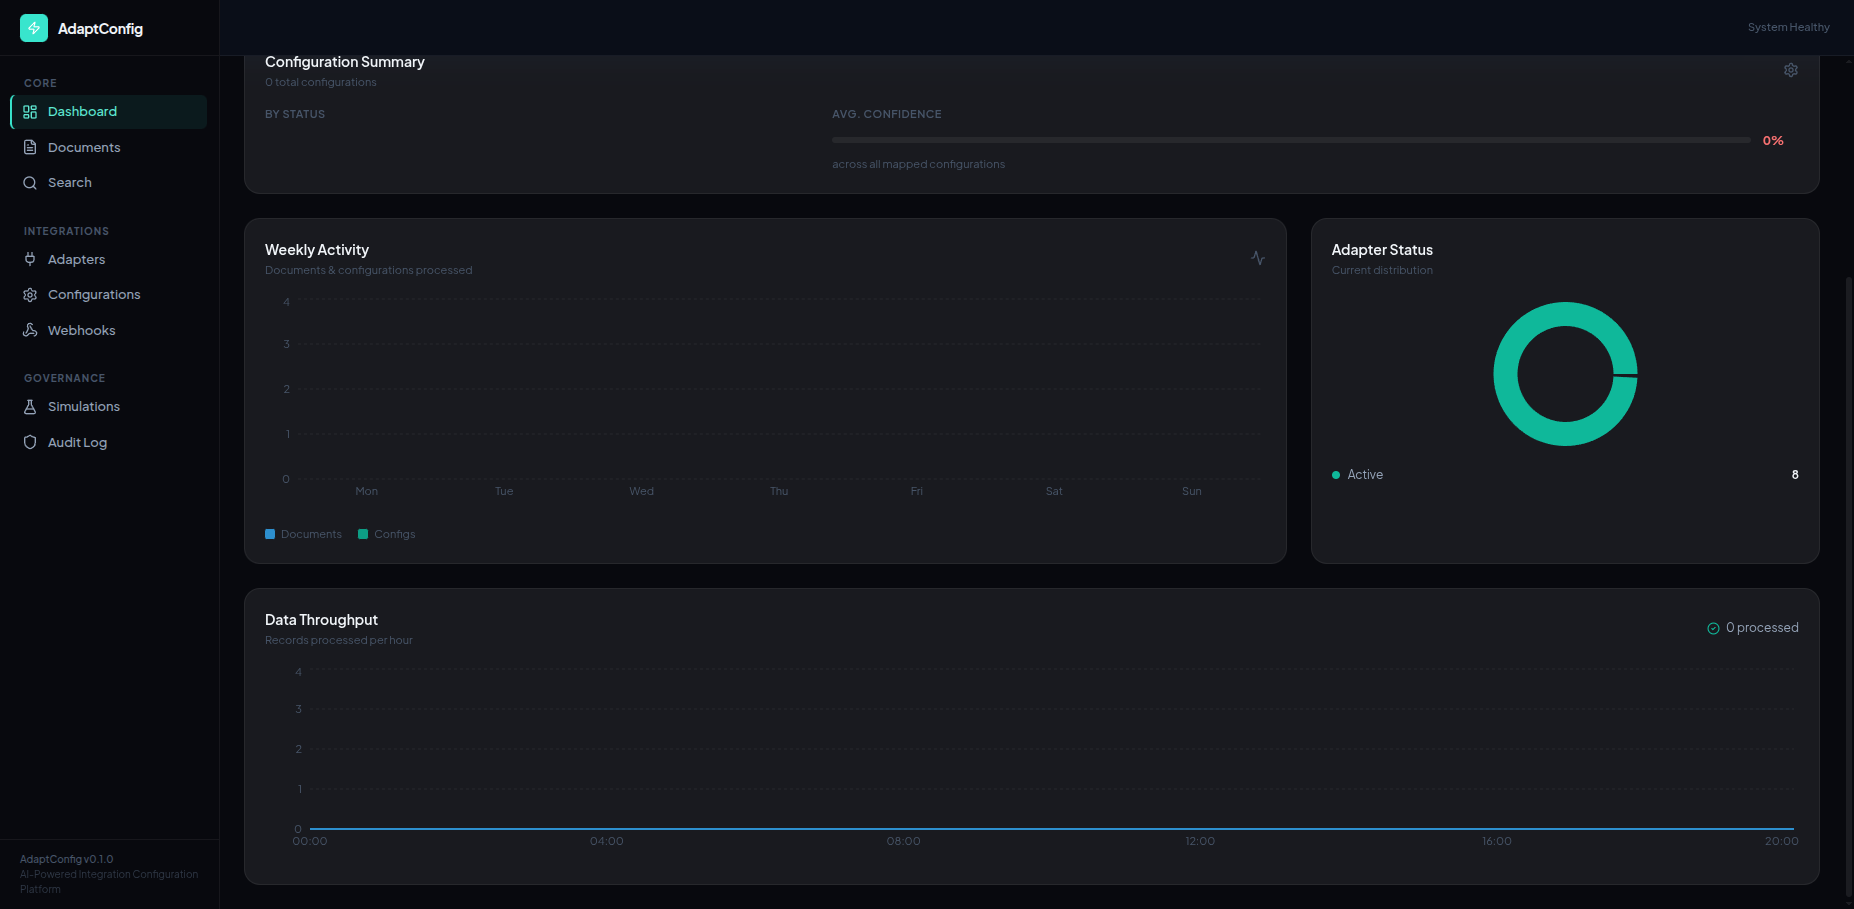
\includegraphics[width=0.88\textwidth]{qa-dashboard-full.png}
\end{center}
\vspace{-0.5em}
{\small Real-time metrics: 8 adapters, configuration summary with confidence scores, weekly activity charts, adapter status distribution.}
\end{frame}

% ══════════════════════════════════════════════════════════════════════════════
% DEMO: STEP 1 — UPLOAD & PARSE
% ══════════════════════════════════════════════════════════════════════════════

\begin{frame}{Step 1: Upload \& Parse Document}
\begin{columns}
\begin{column}{0.55\textwidth}
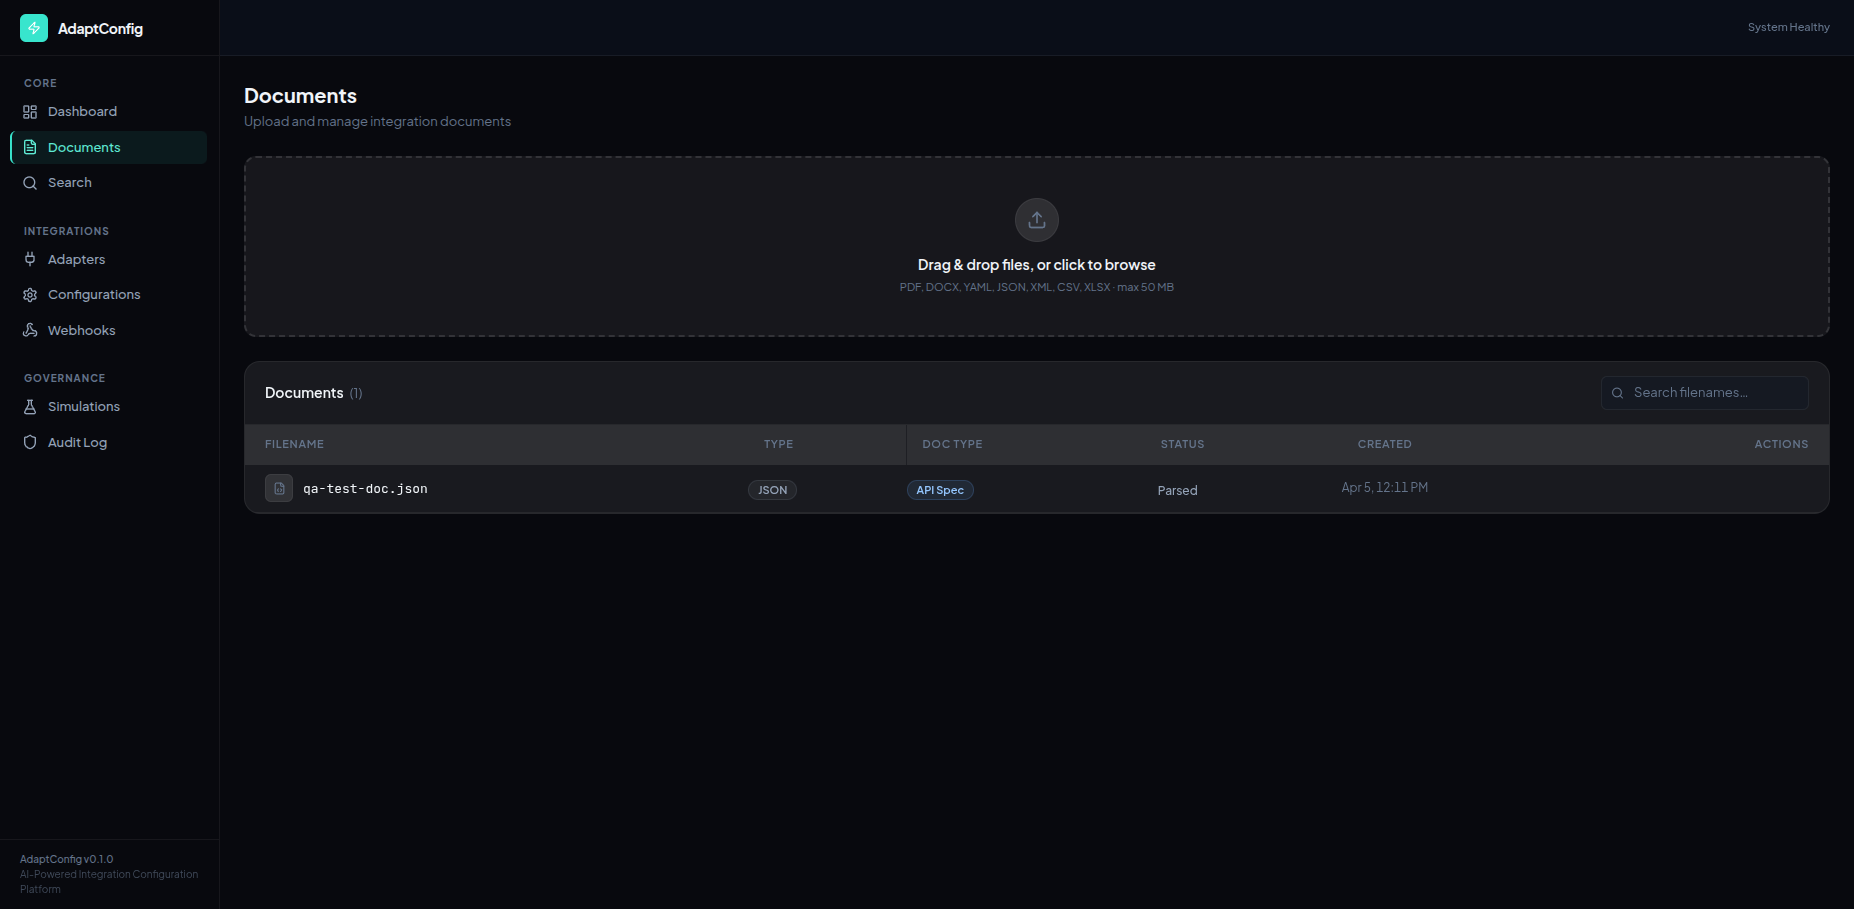
\includegraphics[width=\textwidth]{qa-documents-after-upload.png}
\end{column}
\begin{column}{0.42\textwidth}
\textbf{Supported formats:}
\begin{itemize}
\item OpenAPI YAML / JSON
\item Business Requirements (DOCX, PDF)
\item Any API specification
\end{itemize}

\vspace{0.4em}
\textbf{Parser extracts:}
\begin{itemize}
\item API endpoints \& HTTP methods
\item Request/response fields with types
\item Authentication schemes
\item SLA requirements
\item Base URLs
\end{itemize}

\vspace{0.3em}
{\color{teal}\textbf{95\% confidence}} on CIBIL spec\\
{\small 4 endpoints, 28 fields, 2 auth schemes}
\end{column}
\end{columns}
\end{frame}

% ══════════════════════════════════════════════════════════════════════════════
% DEMO: PARSED DETAIL
% ══════════════════════════════════════════════════════════════════════════════

\begin{frame}{Parsed Document Detail — 5-Tab Modal}
\begin{center}
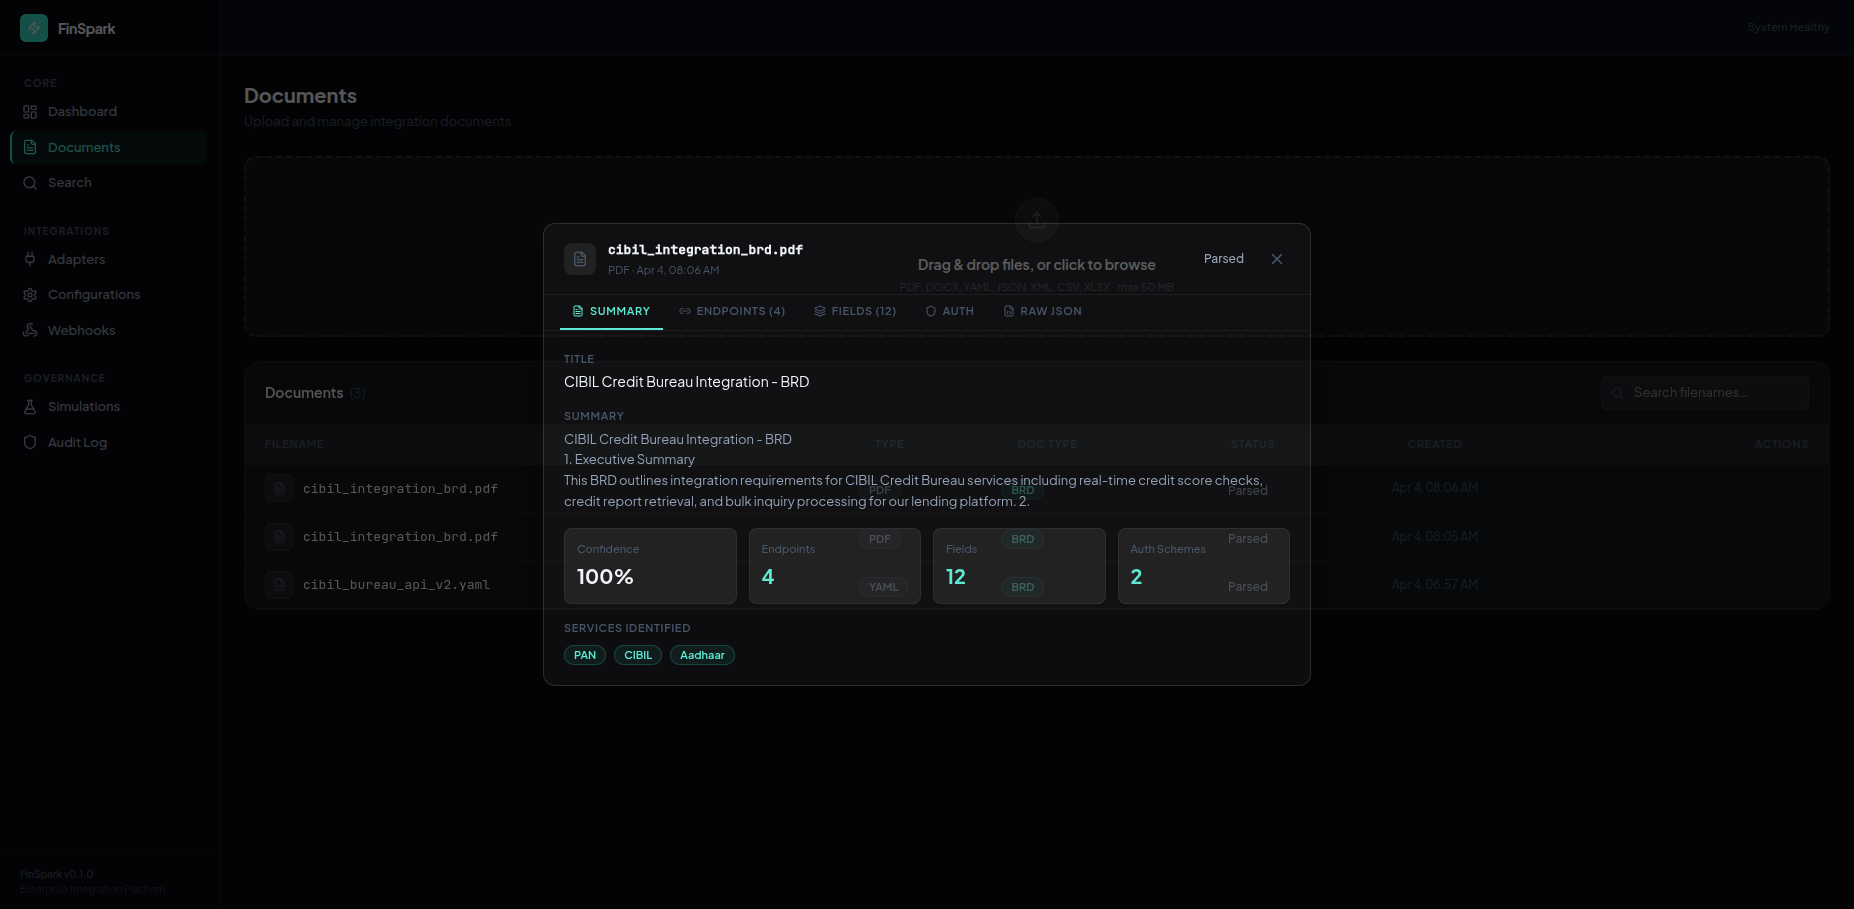
\includegraphics[width=0.82\textwidth]{04-document-detail-modal.png}
\end{center}
\vspace{-0.5em}
{\small \textbf{Summary}: Title, confidence, services identified $\cdot$
\textbf{Endpoints}: Path, method, description $\cdot$
\textbf{Fields}: 28 fields with types \& required flags $\cdot$
\textbf{Auth}: OAuth2 + API Key $\cdot$
\textbf{Raw JSON}: Full parsed output}
\end{frame}

% ══════════════════════════════════════════════════════════════════════════════
% DEMO: STEP 2 — AI CONFIG GENERATION
% ══════════════════════════════════════════════════════════════════════════════

\begin{frame}{Step 2: AI-Powered Configuration Generation}
\begin{columns}
\begin{column}{0.52\textwidth}
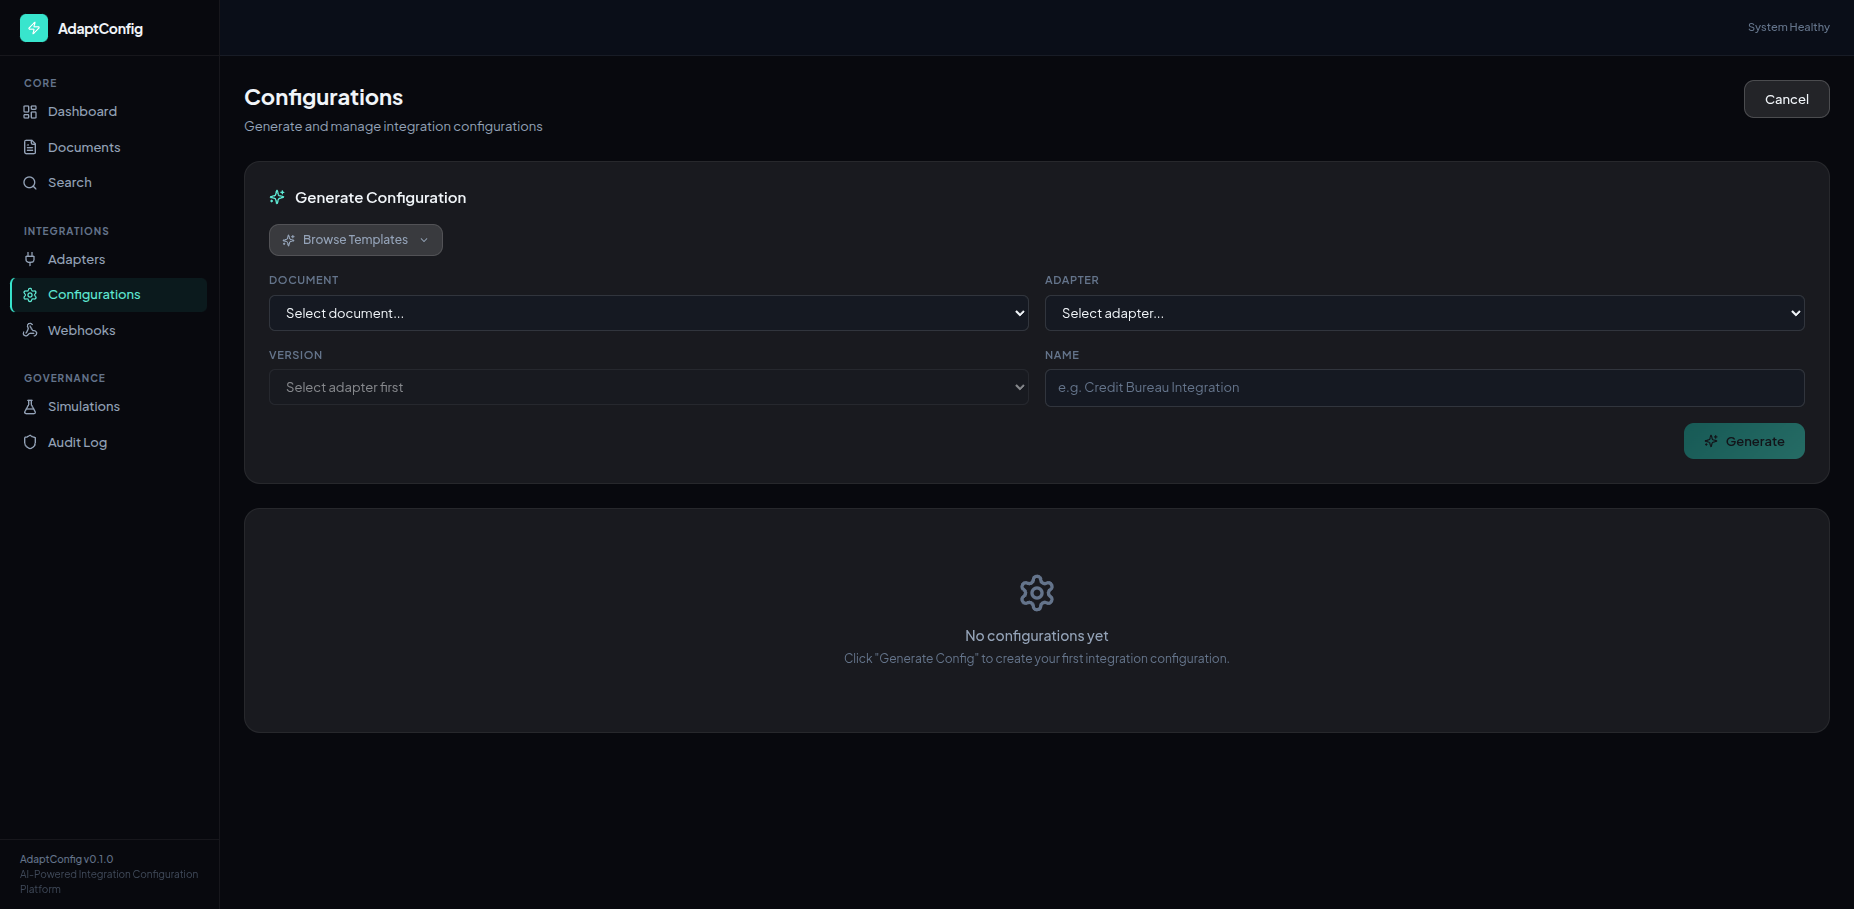
\includegraphics[width=\textwidth]{qa-config-generate-form.png}
\end{column}
\begin{column}{0.44\textwidth}
\textbf{Two-stage AI pipeline:}
\vspace{0.3em}

\begin{enumerate}
\item \textcolor{teal}{\textbf{Gemini 3 Flash}} generates initial config from document entities + adapter schema
\vspace{0.3em}
\item \textbf{Rule-based mapper} augments with:
\begin{itemize}
\item Fuzzy field matching
\item Indian fintech synonym lookup\\(PAN, Aadhaar, GSTIN, IFSC)
\item Confidence scoring
\item Transform suggestions
\end{itemize}
\end{enumerate}

\vspace{0.3em}
\textcolor{success}{\textbf{Result: 28/28 fields mapped at 100\%}}

\vspace{0.3em}
{\small\color{textsecondary} If no matching adapter exists, the system auto-detects and prompts to create one from the parsed spec.}
\end{column}
\end{columns}
\end{frame}

% ══════════════════════════════════════════════════════════════════════════════
% DEMO: FIELD MAPPINGS
% ══════════════════════════════════════════════════════════════════════════════

\begin{frame}{Editable Field Mappings with Confidence}
\begin{center}
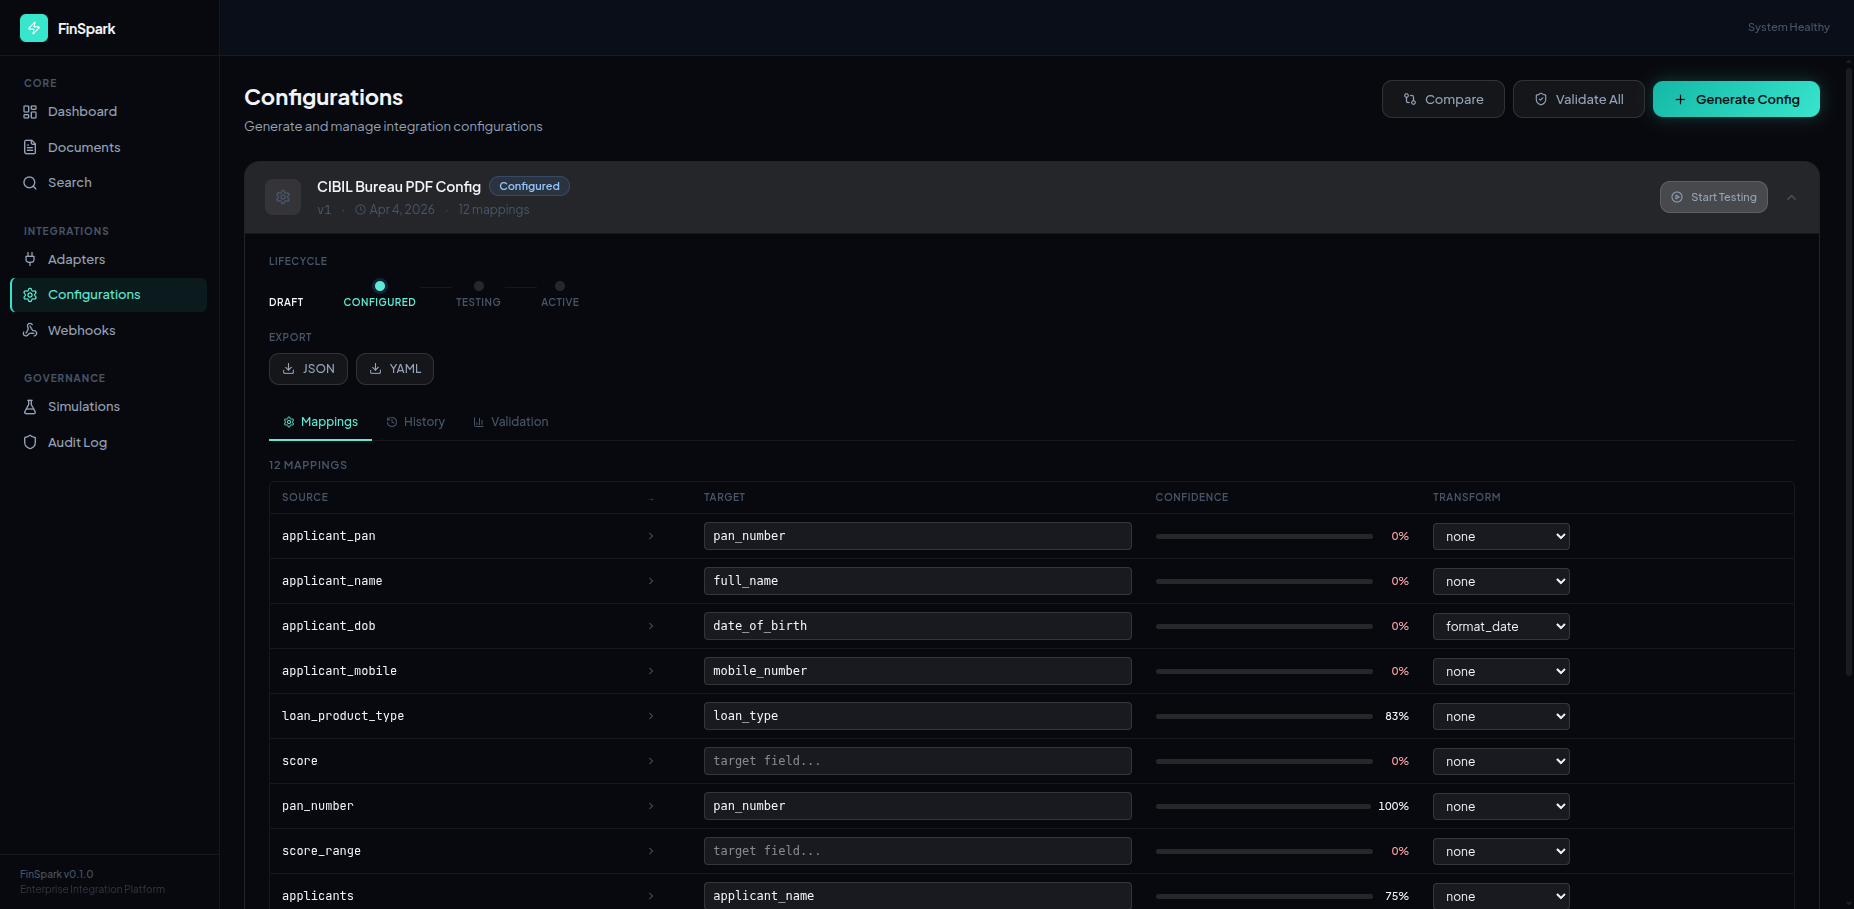
\includegraphics[width=0.88\textwidth]{09-config-generated.png}
\end{center}
\vspace{-0.5em}
{\small Lifecycle stepper (Draft $\to$ Configured $\to$ Validating $\to$ Testing $\to$ Active) $\cdot$
Editable target fields $\cdot$ Transform dropdowns $\cdot$ Color-coded confidence bars $\cdot$
Export JSON/YAML $\cdot$ Version history with rollback}
\end{frame}

% ══════════════════════════════════════════════════════════════════════════════
% DEMO: STEP 3 — SIMULATION
% ══════════════════════════════════════════════════════════════════════════════

\begin{frame}{Step 3: Simulation \& Testing}
\begin{columns}
\begin{column}{0.52\textwidth}
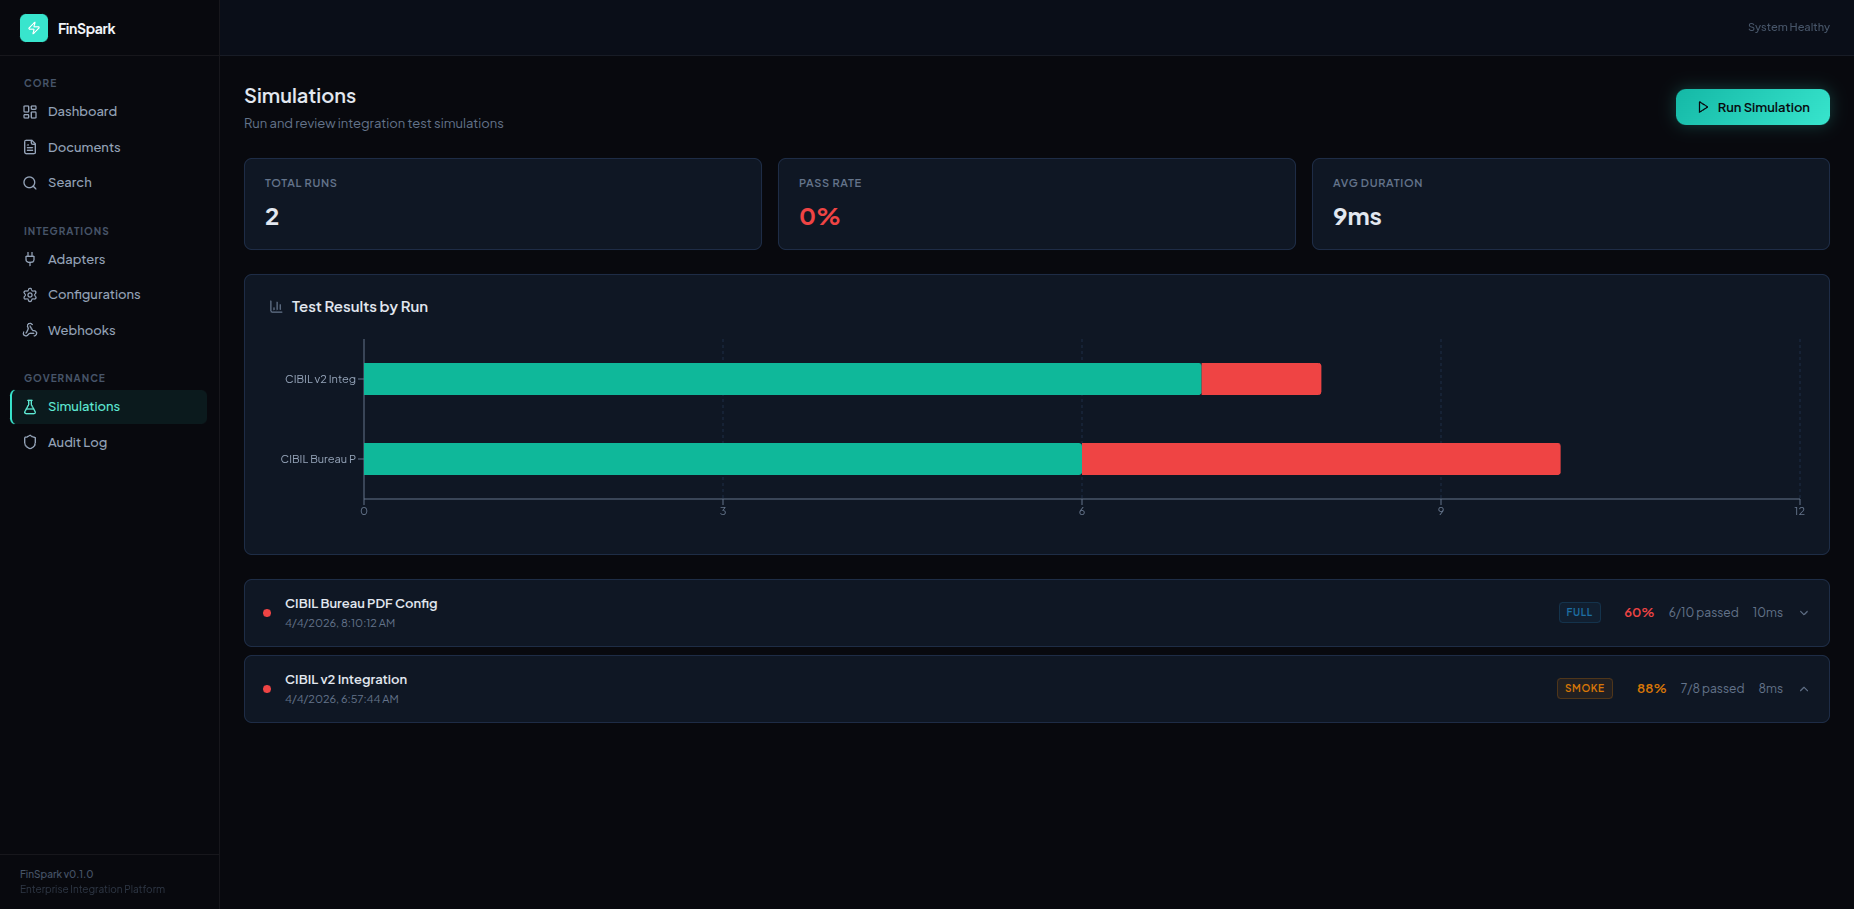
\includegraphics[width=\textwidth]{12-simulation-results.png}
\end{column}
\begin{column}{0.44\textwidth}
\textbf{8-step validation pipeline:}
\vspace{0.3em}

\begin{enumerate}
\item[\textcolor{success}{1.}] Config structure validation
\item[\textcolor{success}{2.}] Field mapping coverage
\item[\textcolor{success}{3.}] Endpoint test: /scores
\item[\textcolor{success}{4.}] Endpoint test: /reports
\item[\textcolor{success}{5.}] Endpoint test: /batch/inquiries
\item[\textcolor{success}{6.}] Endpoint test: /consent/verify
\item[\textcolor{success}{7.}] Auth config validation
\item[\textcolor{success}{8.}] Hooks validation
\end{enumerate}

\vspace{0.3em}
\textcolor{success}{\textbf{8/8 PASSED}}

\vspace{0.3em}
{\small Mock responses generated per adapter with realistic Indian fintech data (CIBIL scores 300--900, UTR numbers, consent artifacts).}
\end{column}
\end{columns}
\end{frame}

% ══════════════════════════════════════════════════════════════════════════════
% ADAPTERS
% ══════════════════════════════════════════════════════════════════════════════

\begin{frame}{Pre-Built Adapter Catalog}
\begin{center}
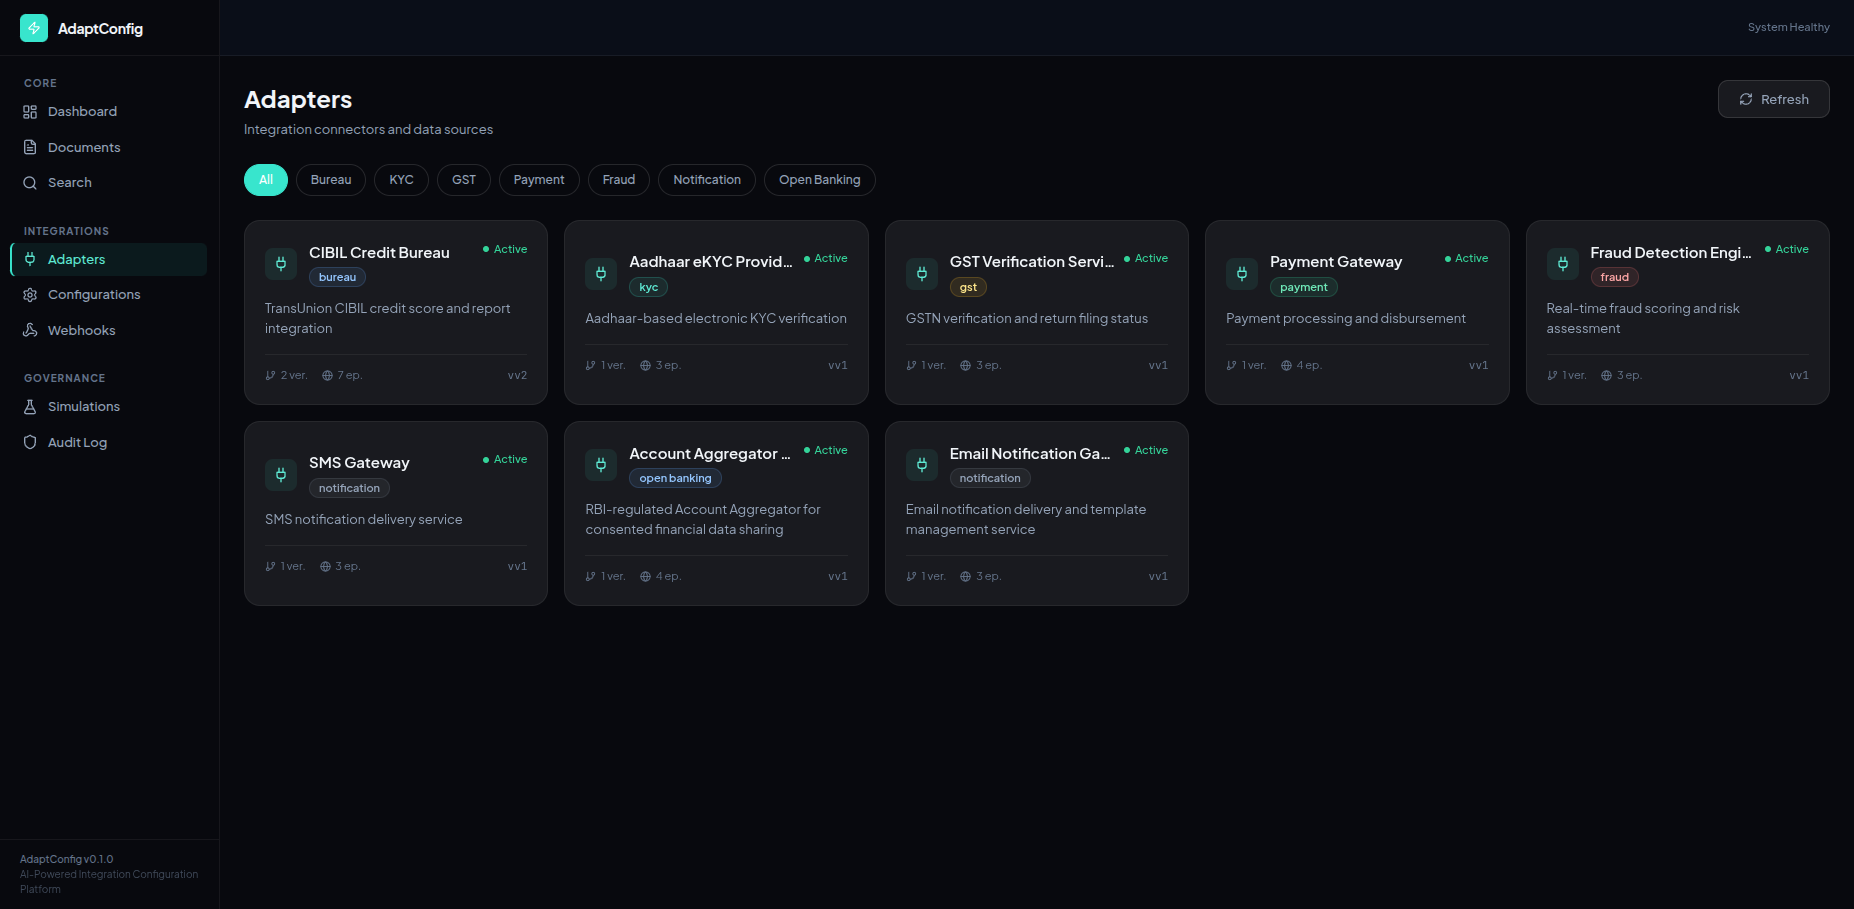
\includegraphics[width=0.88\textwidth]{qa-adapters.png}
\end{center}
\vspace{-0.5em}
{\small 8 adapters: CIBIL (v1+v2), Aadhaar eKYC, GST, Payment Gateway, Fraud Detection, SMS, Account Aggregator (AA), Email $\cdot$ Category filtering $\cdot$ Version details with endpoints $\cdot$ \textbf{Auto-create new adapters from any uploaded API spec}}
\end{frame}

% ══════════════════════════════════════════════════════════════════════════════
% SEARCH
% ══════════════════════════════════════════════════════════════════════════════

\begin{frame}{Cross-Platform Search}
\begin{center}
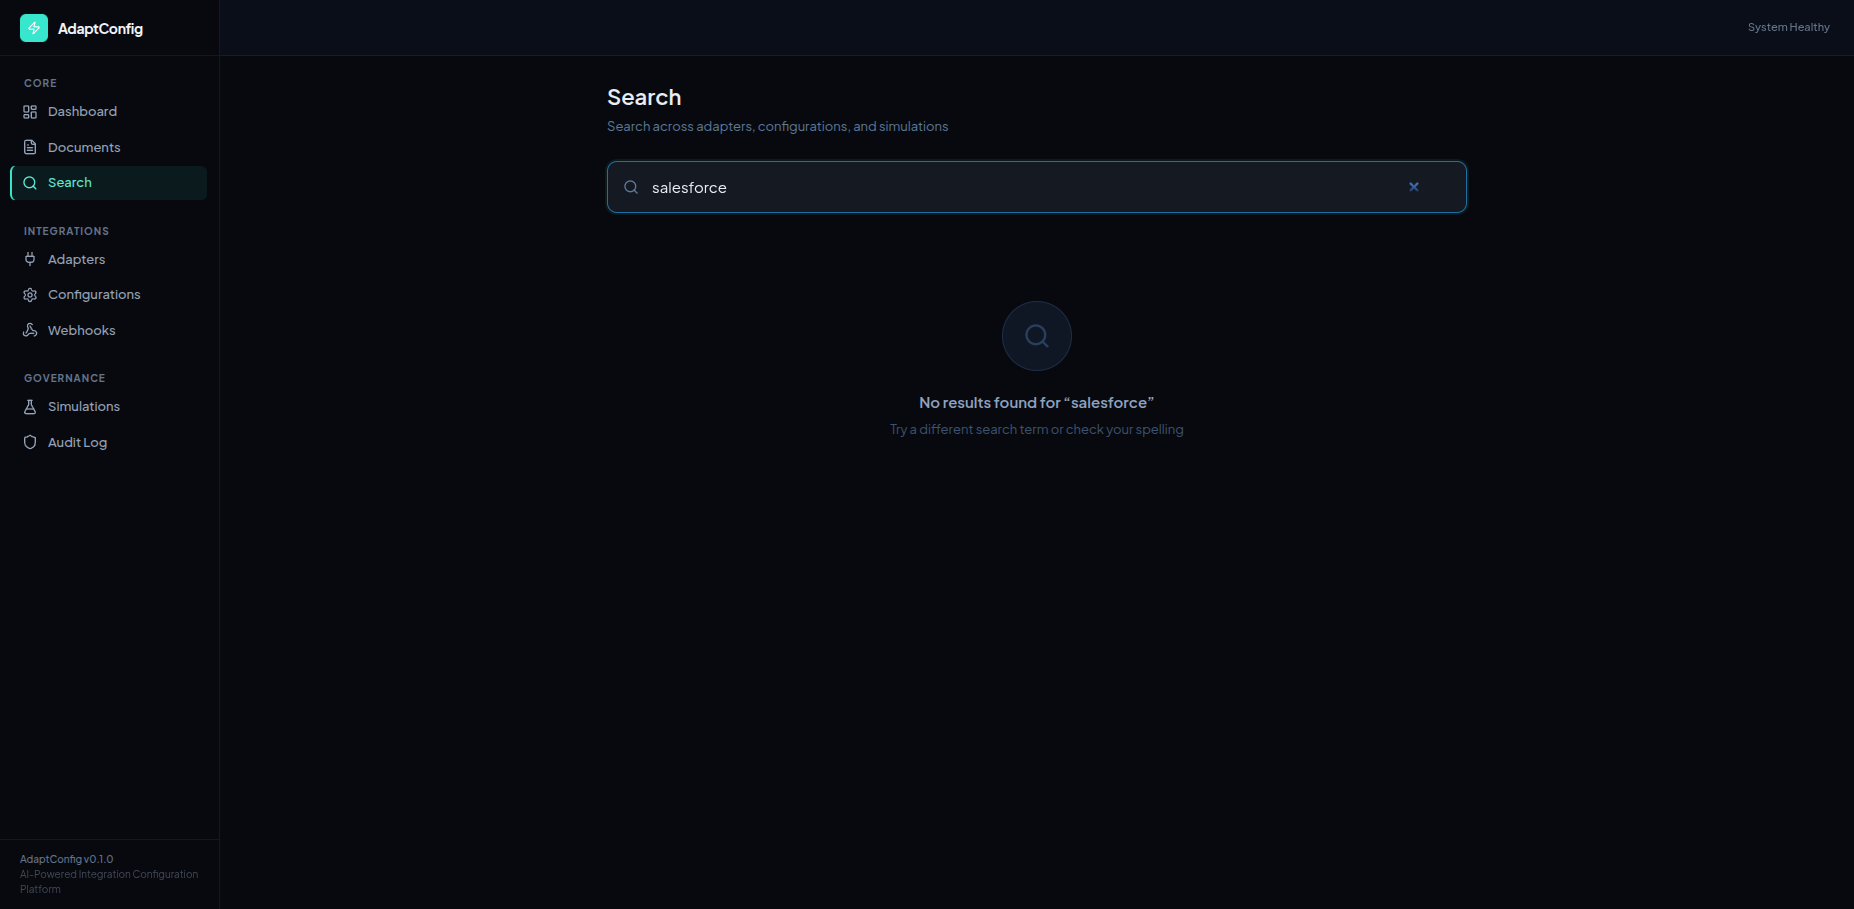
\includegraphics[width=0.75\textwidth]{qa-search-results.png}
\end{center}
\vspace{-0.5em}
{\small Fuzzy search across adapters, configurations, and simulations $\cdot$ Results grouped by type with relevance scores $\cdot$ Debounced real-time results}
\end{frame}

% ══════════════════════════════════════════════════════════════════════════════
% AUDIT + WEBHOOKS
% ══════════════════════════════════════════════════════════════════════════════

\begin{frame}{Governance: Audit Trail \& Webhooks}
\begin{columns}
\begin{column}{0.52\textwidth}
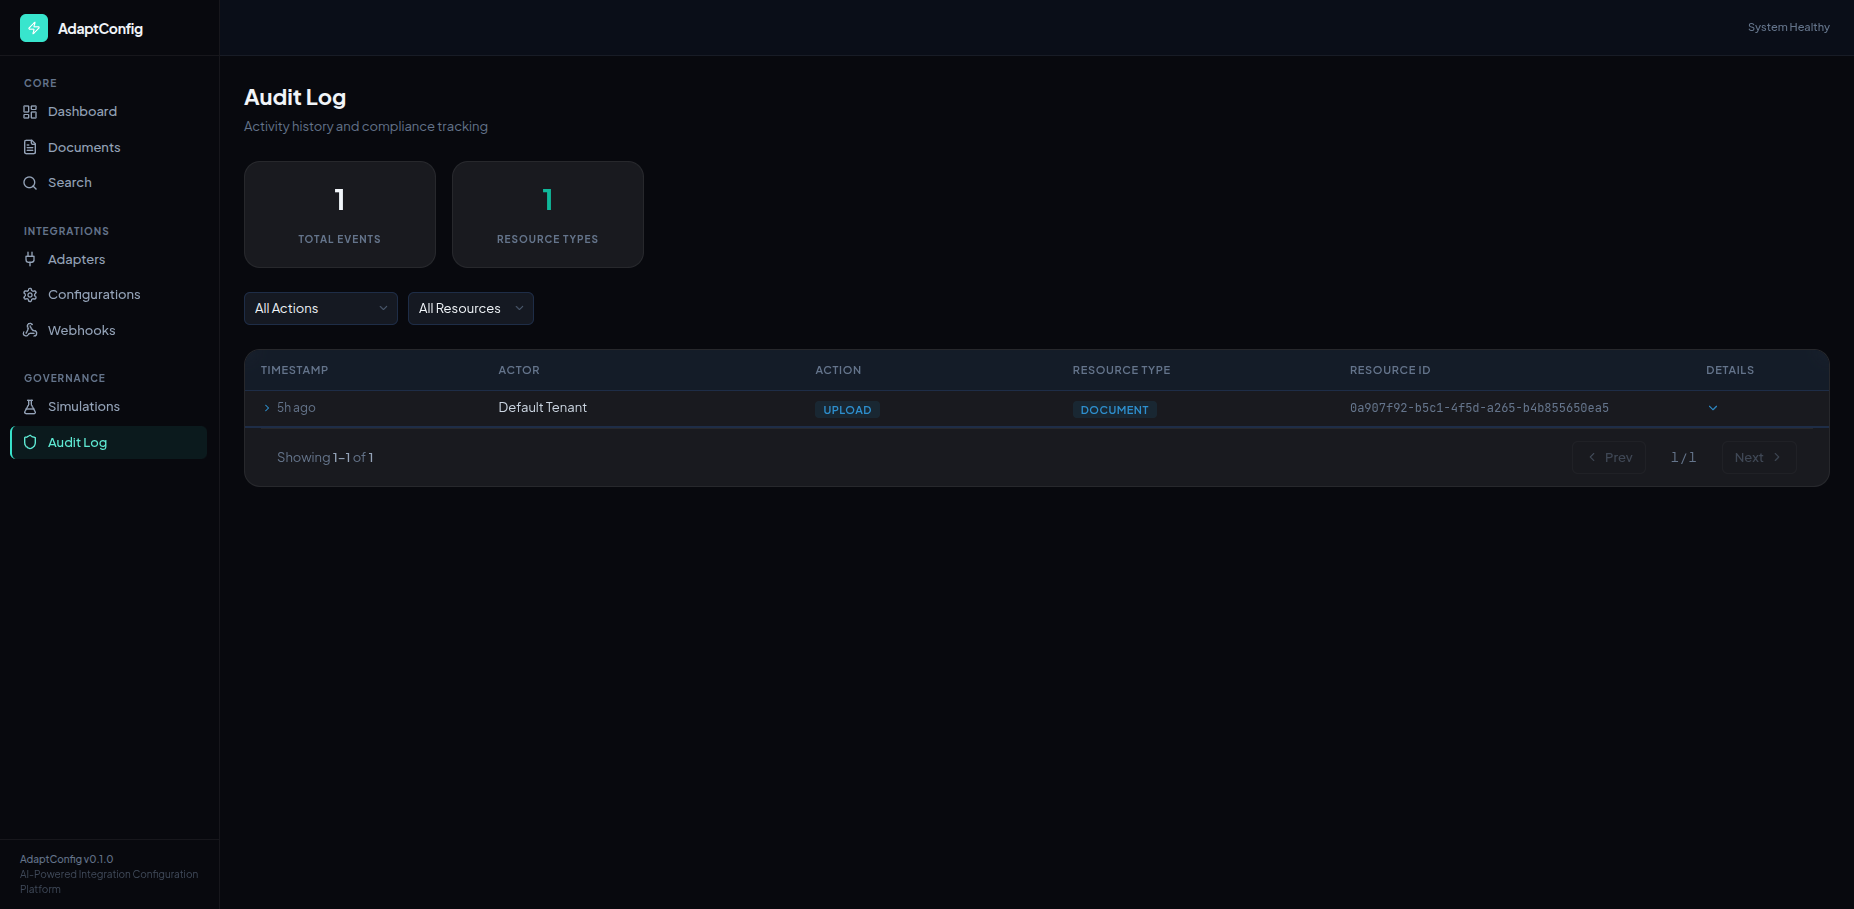
\includegraphics[width=\textwidth]{qa-audit.png}
\vspace{0.2em}
{\scriptsize\textbf{Audit Log}: Immutable trail of all actions with filters and pagination}
\end{column}
\begin{column}{0.44\textwidth}
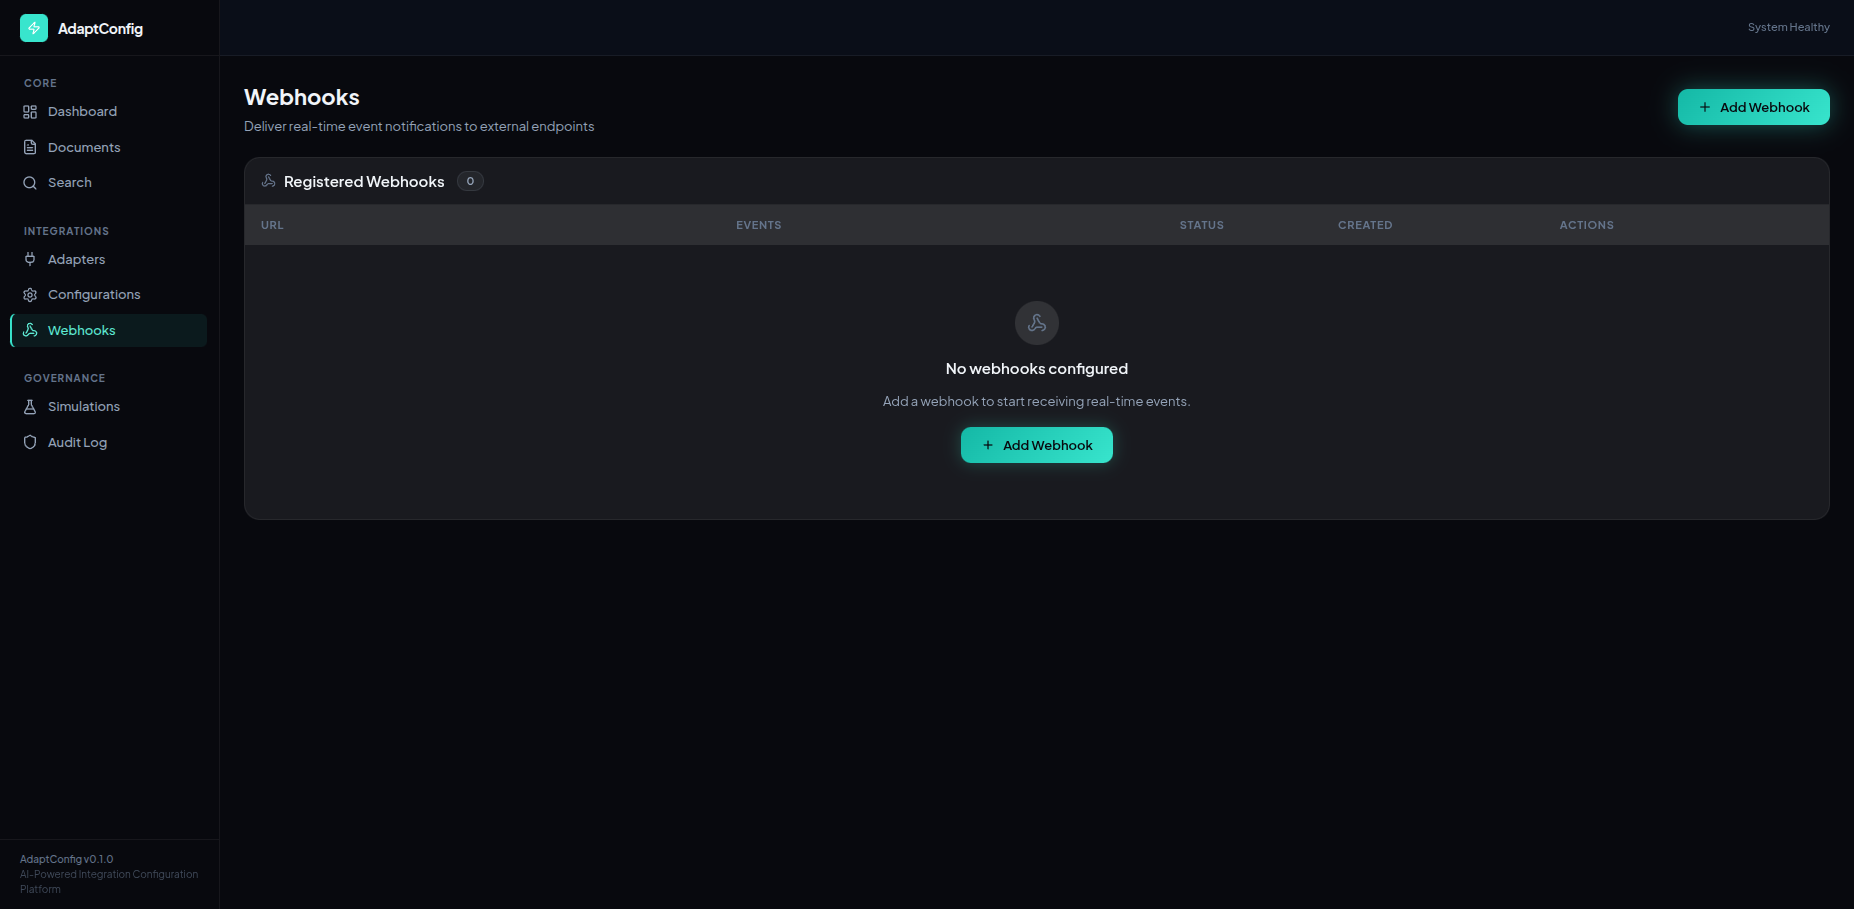
\includegraphics[width=\textwidth]{qa-webhooks.png}
\vspace{0.2em}
{\scriptsize\textbf{Webhooks}: Register URLs for event callbacks, test delivery, manage subscriptions}
\end{column}
\end{columns}
\end{frame}

% ══════════════════════════════════════════════════════════════════════════════
% SECURITY
% ══════════════════════════════════════════════════════════════════════════════

\begin{frame}{Security \& Compliance}
\begin{columns}[T]
\begin{column}{0.48\textwidth}
\begin{block}{Authentication}
\begin{itemize}
\item JWT Bearer tokens (HS256)
\item PBKDF2 + salt password hashing
\item Token refresh flow
\item RBAC (admin / editor / viewer)
\end{itemize}
\end{block}

\begin{block}{Data Protection}
\begin{itemize}
\item Per-user tenant isolation
\item PII masking (Aadhaar, PAN, phone)
\item AES-256 Fernet encryption
\item Path traversal protection
\item File size \& type validation
\end{itemize}
\end{block}
\end{column}
\begin{column}{0.48\textwidth}
\begin{block}{Infrastructure}
\begin{itemize}
\item CORS restricted to known origins
\item CSP, HSTS, X-Frame headers
\item Rate limiting (100 req/min)
\item Structured JSON logging
\item Graceful shutdown (30s drain)
\item Alembic database migrations
\end{itemize}
\end{block}

\begin{block}{Testing}
\begin{itemize}
\item \textbf{899 automated tests}
\item \textbf{82\% code coverage}
\item Unit + integration + E2E
\item Production deployed on Railway
\end{itemize}
\end{block}
\end{column}
\end{columns}
\end{frame}

% ══════════════════════════════════════════════════════════════════════════════
% KEY FEATURES
% ══════════════════════════════════════════════════════════════════════════════

\begin{frame}{Key Features Summary}
\begin{center}
\begin{tabular}{p{3.5cm}p{9cm}}
\toprule
\textbf{Category} & \textbf{Features} \\
\midrule
\textbf{Parsing} & PDF, DOCX, YAML, JSON $\cdot$ endpoints, fields, auth extraction $\cdot$ confidence scoring \\[4pt]
\textbf{AI Config} & Gemini 3 Flash $\cdot$ fuzzy field matching $\cdot$ Indian fintech synonyms $\cdot$ transform suggestions \\[4pt]
\textbf{Adapters} & 8 pre-built $\cdot$ auto-create from any API spec $\cdot$ category filtering $\cdot$ versioning \\[4pt]
\textbf{Simulation} & 8-step validation $\cdot$ mock responses per adapter $\cdot$ step-by-step results \\[4pt]
\textbf{Lifecycle} & Draft $\to$ Configured $\to$ Validating $\to$ Testing $\to$ Active $\cdot$ rollback $\cdot$ history \\[4pt]
\textbf{Security} & JWT auth $\cdot$ per-user isolation $\cdot$ PII masking $\cdot$ rate limiting $\cdot$ CORS \\[4pt]
\textbf{UX} & Glassmorphism theme $\cdot$ 8 pages $\cdot$ search $\cdot$ webhooks $\cdot$ audit $\cdot$ pagination \\
\bottomrule
\end{tabular}
\end{center}
\end{frame}

% ══════════════════════════════════════════════════════════════════════════════
% RESULTS
% ══════════════════════════════════════════════════════════════════════════════

\begin{frame}{Results \& Metrics}
\begin{columns}[T]
\begin{column}{0.48\textwidth}
\begin{center}
\begin{tabular}{lr}
\toprule
\textbf{Metric} & \textbf{Value} \\
\midrule
API Endpoints & 34 \\
Pre-built Adapters & 8 \\
Automated Tests & 899 \\
Code Coverage & 82\% \\
Frontend Pages & 8 \\
Lines of Code & $\sim$15,000 \\
\bottomrule
\end{tabular}
\end{center}
\end{column}
\begin{column}{0.48\textwidth}
\begin{center}
\begin{tabular}{lr}
\toprule
\textbf{Performance} & \textbf{Value} \\
\midrule
Parse confidence & 95\% \\
Mapping accuracy & 100\% \\
Simulation pass & 8/8 \\
Config gen time & $<$ 5s \\
Doc parse time & $<$ 1s \\
Test suite time & $\sim$110s \\
\bottomrule
\end{tabular}
\end{center}
\end{column}
\end{columns}

\vspace{0.8em}
\begin{center}
\begin{tabular}{lccc}
\toprule
& \textbf{Manual} & \textbf{AdaptConfig} & \textbf{Improvement} \\
\midrule
Time per integration & 2--4 weeks & $<$ 5 minutes & \textcolor{success}{$\sim$500x faster} \\
Field mapping errors & Common & AI-validated & \textcolor{success}{Near zero} \\
Pre-deploy testing & Rarely done & Always & \textcolor{success}{8-step pipeline} \\
Cost per platform & Rs 48--96L & Minimal & \textcolor{success}{$>$95\% savings} \\
\bottomrule
\end{tabular}
\end{center}
\end{frame}

% ══════════════════════════════════════════════════════════════════════════════
% LIVE DEMO
% ══════════════════════════════════════════════════════════════════════════════

\begin{frame}{Live Demo}
\begin{center}
{\Large\textbf{Live at:} \textcolor{teal}{\url{https://adaptconfig-frontend-production.up.railway.app}}}

\vspace{1em}

\begin{tikzpicture}[
    node distance=0.55cm,
    step/.style={rectangle, draw=teal!60, fill=surface, text=textprimary,
                 rounded corners=4pt, minimum height=0.65cm, minimum width=8cm,
                 font=\small},
    arrow/.style={->, thick, teal!60}
]
    \node[step] (s1) {1. Register / Login};
    \node[step, below=of s1] (s2) {2. Upload CIBIL API Spec (YAML)};
    \node[step, below=of s2] (s3) {3. View Parsed Fields (28 fields, 4 endpoints, 2 auth)};
    \node[step, below=of s3] (s4) {4. Generate Config (Gemini 3 + Rule Engine)};
    \node[step, below=of s4] (s5) {5. Review Field Mappings (100\% confidence)};
    \node[step, below=of s5] (s6) {6. Validate \& Simulate (8/8 PASS)};
    \node[step, below=of s6] (s7) {7. Lifecycle: Configured $\to$ Validating $\to$ Testing $\to$ Active};

    \draw[arrow] (s1) -- (s2);
    \draw[arrow] (s2) -- (s3);
    \draw[arrow] (s3) -- (s4);
    \draw[arrow] (s4) -- (s5);
    \draw[arrow] (s5) -- (s6);
    \draw[arrow] (s6) -- (s7);
\end{tikzpicture}
\end{center}
\end{frame}

% ══════════════════════════════════════════════════════════════════════════════
% THANK YOU
% ══════════════════════════════════════════════════════════════════════════════

\begin{frame}[plain]
\begin{center}
\vspace{2cm}
{\Huge\bfseries Thank You}

\vspace{0.8em}
{\Large\color{teal} AdaptConfig}

\vspace{0.3em}
{\color{textsecondary} AI-Powered Integration Configuration Platform}

\vspace{1.5em}

{\small
\begin{tabular}{rl}
\textcolor{teal}{Live App} & \url{https://adaptconfig-frontend-production.up.railway.app} \\
\textcolor{teal}{API Docs} & \url{https://adaptconfig-api-production.up.railway.app/docs} \\
\textcolor{teal}{GitHub} & \url{https://github.com/Akasxh/adaptconfig} \\
\end{tabular}
}

\vspace{1em}
{\color{textsecondary}\small Team Nucleolus $\cdot$ S Akash $\cdot$ Swayam Jain $\cdot$ Yash Kamdar $\cdot$ IIT Patna}
\end{center}
\end{frame}

\end{document}
